\section{二元信道的容量}
\label{sec:dcc-binary}

翻转与擦除是二元输入上最基本的两种损坏。它们的容量各是多少？损坏的概率相同时，哪一种更伤害传输？两个信道都有一个对称性：把输入的$0$与$1$互换，同时把输出的$0$与$1$互换（擦除符号不动），转移矩阵不变。

对称性给出最优输入的候选。若$q$是最优输入分布，把它的两个分量互换得到$\tilde{q}$，由于信道在互换下不变，$I(\tilde{q})=I(q)=C$。由定理~\ref{thm:dcc-capacity-exists}，最优输入组成凸集，所以$\tfrac12q+\tfrac12\tilde{q}=(\tfrac12,\tfrac12)$也最优。于是两个信道的容量都在均匀输入处取到。下面直接算出这个值，再用上界~\eqref{eq:dcc-upper-bound}独立核验。

\subsection{二元对称信道}
\label{sec:dcc-bsc}

设翻转概率为$p\in[0,1]$。给定任一输入，输出是“翻”或“不翻”的二选一，概率为$p$与$1-p$，条件熵是二元熵$h_2(p)$，与输入分布无关：
\[
 H(Y\mid X)=\sum_xq(x)H(W_x)=h_2(p) .
\]
所以互信息只通过输出熵依赖输入分布：
\[
 I(q)=H(Y)-h_2(p)\leq1-h_2(p) ,
\]
因为$Y$只取两个值，$H(Y)\leq1$。均匀输入时，$p_q(1)=\tfrac12(1-p)+\tfrac12p=\tfrac12$，输出均匀，$H(Y)=1$，等号成立。于是
\begin{equation}
 C_{\mathrm{BSC}}(p)=1-h_2(p) .
 \label{eq:dcc-bsc-capacity}
\end{equation}

用式~\eqref{eq:dcc-upper-bound}核验：取$r=(\tfrac12,\tfrac12)$，两行到$r$的散度相同，
\[
 D_{\mathrm{KL}}(W_0\Vert r)=(1-p)\log_2\bigl(2(1-p)\bigr)+p\log_2(2p)=1-h_2(p) ,
\]
$W_1$的计算只是交换两项。所以$C\leq1-h_2(p)$，而均匀输入达到这个值。这一核验不依赖对称性论证，也说明条件~\eqref{eq:dcc-kkt}在均匀输入处成立。

$p=0.1$时，
\[
 h_2(0.1)=0.1\log_210+0.9\log_2\tfrac{10}{9}\approx0.469 ,
\]
容量约为$0.531$比特每次使用。三次重复码以码率$\tfrac13$达到$0.028$的错误；编码定理说，用足够长的码，码率可以接近$0.531$而错误仍趋于零。

\paragraph{端点}
$p=0$时信道无噪声，$C=1$。$p=\tfrac12$时输出与输入独立，无论发什么，接收端看到的都是公平硬币，$C=0$。$p=1$时每个符号都被翻转，但翻转是确定的，接收端把收到的符号全部取反就能完全恢复，$C=1-h_2(1)=1$。所以“翻转发生”与“信息损失”不是一回事：损失来自不知道哪些符号被翻转，即翻转的不可预测性。$h_2(p)$关于$p=\tfrac12$对称，翻转概率$0.9$与$0.1$的信道容量相同。

\subsection{二元擦除信道}
\label{sec:dcc-bec}

设擦除概率为$\varepsilon\in[0,1]$，输出取$0$、$\mathrm{e}$、$1$。这里换一个分解更方便：$I(X;Y)=H(X)-H(X\mid Y)$，计算接收端看到输出后对输入还剩多少不确定性。

看到$0$或$1$时，输入就是这个值，没有剩余的不确定性。看到$\mathrm{e}$时，因为擦除与输入无关，
\[
 \mathbb{P}(X=x\mid Y=\mathrm{e})=\frac{q(x)\varepsilon}{\varepsilon}=q(x) ,
\]
输入仍是原来的分布，剩余$H(X)$。$Y=\mathrm{e}$的概率是$\varepsilon$，所以$H(X\mid Y)=\varepsilon H(X)$，并且
\[
 I(q)=(1-\varepsilon)H(X)\leq1-\varepsilon .
\]
均匀输入使$H(X)=1$，等号成立：
\begin{equation}
 C_{\mathrm{BEC}}(\varepsilon)=1-\varepsilon .
 \label{eq:dcc-bec-capacity}
\end{equation}
这个结果有直接的读法：平均有比例$1-\varepsilon$的符号原样到达，每个携带一比特，被擦除的符号什么也不携带。

核验上界：均匀输入的输出分布是
\[
 r=\Bigl(\frac{1-\varepsilon}2,\ \varepsilon,\ \frac{1-\varepsilon}2\Bigr) ,
\]
第一行到它的散度为
\[
 D_{\mathrm{KL}}(W_0\Vert r)=(1-\varepsilon)\log_2\frac{1-\varepsilon}{(1-\varepsilon)/2}+\varepsilon\log_2\frac{\varepsilon}{\varepsilon}=1-\varepsilon ,
\]
第二行相同（$0<\varepsilon<1$；$\varepsilon=1$时两行都是集中在$\mathrm{e}$上的分布，散度为$0$）。由式~\eqref{eq:dcc-upper-bound}，$C\leq1-\varepsilon$。端点$\varepsilon=0$给出无噪声信道的$1$，$\varepsilon=1$时什么也收不到，容量为$0$。

\paragraph{已知错误位置的价值}
比较损坏概率相同的两个信道。图~\ref{fig:dcc-flip-vs-erasure}把同一个输入块分别送进两个信道，在同样两个位置发生损坏。擦除信道的接收端看到$\mathrm{e}$，确切知道哪里缺了信息，其余位置完全可信；对称信道的接收端看到的是普通的$0$和$1$，不知道哪两位是错的，每一位都只能部分相信。

\begin{BookInlineFigure}
 \centering
 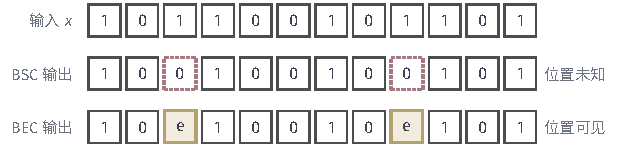
\includegraphics[width=104.5mm]{figures/07-probability/06-channel-coding/tikz/dcc-flip-vs-erasure/figure.pdf}
 \caption{同一个$12$位输入块在第$3$、$9$位受到损坏。二元对称信道把这两位翻转，结果看起来与其他位无异，红色虚线框只是标给读者看的；二元擦除信道把这两位变成可见的擦除符号$\mathrm{e}$（黄色）。}
 \label{fig:dcc-flip-vs-erasure}
\end{BookInlineFigure}

图~\ref{fig:dcc-capacity-curves}比较两条容量曲线。损坏概率都是$0.1$时，擦除信道的容量是$0.9$，对称信道只有$0.531$。差值$h_2(p)-p$可以理解为找出错误位置的代价：在$n$个符号中指出约$np$个翻转位置，需要约$nh_2(p)$比特的描述，而擦除信道把这些位置免费告诉了接收端，只损失被擦掉的$np$比特本身。对$0<p<\tfrac12$总有$h_2(p)>p$，所以未知的翻转总比可见的擦除更伤害传输。

\begin{BookInlineFigure}
 \centering
 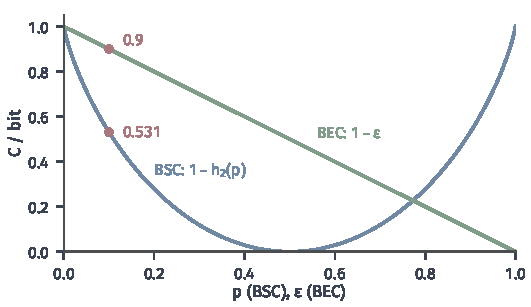
\includegraphics[width=90mm]{figures/07-probability/06-channel-coding/matplotlib/dcc-capacity-curves/figure.pdf}
 \caption{二元对称信道的容量$1-h_2(p)$（蓝）与二元擦除信道的容量$1-\varepsilon$（绿），横轴为翻转概率或擦除概率。红点标出损坏概率$0.1$时的两个容量$0.531$与$0.9$。蓝线关于$p=\tfrac12$对称：确定的翻转不损失信息。}
 \label{fig:dcc-capacity-curves}
\end{BookInlineFigure}

\paragraph{对称性的作用}
两个信道的均匀输入最优，依赖的是交换$0$与$1$的对称性，不是二元输入本身。第~\ref{sec:dcc-capacity-formula}节的Z信道同样是二元输入，却没有这种对称性：输入$1$会出错而输入$0$不会，最优输入是$q=0.4$，均匀输入少得约$0.011$比特。对一般的转移矩阵，最优输入要从条件~\eqref{eq:dcc-kkt}解出，通常没有闭式，这就需要第~\ref{sec:dcc-numerical}节的数值方法。
